% Gabarit pandoc des corrigés publiés (brut et guidé). Contenu sans marque ni nom de site.
% Compilation : lualatex (latexmk -lualatex).
% Le Markdown reste la source unique : ne pas éditer ce fichier .tex à la main.
\documentclass[11pt,a4paper]{article}

% --- Moteur, polices (Latin Modern) et langue ---------------------------------
\usepackage{iftex}
\ifLuaTeX\else\errmessage{Ce document se compile avec lualatex}\fi
\usepackage{amsmath,amssymb,mathtools}
\usepackage{fontspec}
% mathrm=sym : \mathrm prend ses glyphes dans la police mathématique (ℓ, μ, Ω), comme KaTeX.
\usepackage[math-style=TeX,bold-style=TeX,mathrm=sym]{unicode-math}
% Repli pour les glyphes absents de Latin Modern (indices et exposants Unicode,
% flèches, filets des schémas en texte, symboles) : DejaVu, puis Latin Modern Math
% (ℓ, lettres mathématiques Unicode des légendes).
\directlua{
  luaotfload.add_fallback("repliTexte", {"DejaVuSerif:mode=harf;", "DejaVuSans:mode=harf;", "file:latinmodern-math.otf:mode=harf;"})
  luaotfload.add_fallback("repliMono", {"DejaVuSansMono:mode=harf;", "DejaVuSans:mode=harf;", "file:latinmodern-math.otf:mode=harf;"})
}
\setmainfont{Latin Modern Roman}[RawFeature={fallback=repliTexte}]
\setsansfont{Latin Modern Sans}[RawFeature={fallback=repliTexte}]
\setmonofont{Latin Modern Mono}[RawFeature={fallback=repliMono}]
\setmathfont{Latin Modern Math}
\usepackage[french]{babel}
\frenchsetup{SmallCapsFigTabCaptions=false}

% --- Mise en page --------------------------------------------------------------
\usepackage[a4paper,margin=2.2cm,headheight=14pt,footskip=1.2cm]{geometry}
\usepackage{microtype}
\setlength{\emergencystretch}{4em}
\tolerance=1500
\setlength{\parindent}{0pt}
\setlength{\parskip}{0.55\baselineskip plus 2pt minus 1pt}
\usepackage{xcolor}
% Gris nommés : babel-french rend « ! » actif dans le document.
\definecolor{gris2}{gray}{0.98}
\definecolor{gris3}{gray}{0.97}
\definecolor{gris5}{gray}{0.95}
\definecolor{gris35}{gray}{0.65}
\definecolor{gris40}{gray}{0.60}
\definecolor{gris45}{gray}{0.55}
\definecolor{gris50}{gray}{0.50}
\definecolor{gris55}{gray}{0.45}
\definecolor{gris60}{gray}{0.40}
\definecolor{gris65}{gray}{0.35}
\definecolor{gris70}{gray}{0.30}
\definecolor{gris80}{gray}{0.20}
\definecolor{gris85}{gray}{0.15}
\usepackage{graphicx}
\usepackage{float}
\usepackage{caption}
\captionsetup{font=small,labelformat=empty,justification=centering}
\usepackage{booktabs,longtable,array,multirow,calc}
\usepackage{siunitx}
\sisetup{locale=FR}
\usepackage[version=4]{mhchem}
\usepackage{listings}
\usepackage{fancyhdr}
\usepackage{lastpage}
\usepackage[most]{tcolorbox}
\usepackage{enumitem}
\setlist{nosep,leftmargin=*,topsep=2pt}
\usepackage[hidelinks,unicode]{hyperref}
\usepackage{bookmark}
\hypersetup{pdftitle={Centrale-Supélec PSI — Mathématiques 2 2026},pdfauthor={Rédigé par IA},pdfcreator={LaTeX},pdfsubject={Corrigé guidé}}
\usepackage{xurl}

% --- Pandoc : listes, tableaux, figures ----------------------------------------
\providecommand{\passthrough}[1]{#1}
\providecommand{\tightlist}{\setlength{\itemsep}{0pt}\setlength{\parskip}{0pt}}

\makeatletter
\def\maxwidth{\ifdim\Gin@nat@width>\linewidth\linewidth\else\Gin@nat@width\fi}
\def\maxheight{\ifdim\Gin@nat@height>0.55\textheight 0.55\textheight\else\Gin@nat@height\fi}
\makeatother
\setkeys{Gin}{width=\maxwidth,height=\maxheight,keepaspectratio}
\setcounter{secnumdepth}{-\maxdimen}
\providecommand{\pandocbounded}[1]{#1}
\usepackage{longtable,booktabs,array}

% --- Code (listings) -----------------------------------------------------------
\lstset{
  basicstyle=\ttfamily\small,
  columns=fullflexible,
  keepspaces=true,
  breaklines=true,
  breakatwhitespace=false,
  postbreak=\mbox{\textcolor{gris50}{$\hookrightarrow$}\space},
  frame=single,
  rulecolor=\color{gris35},
  framesep=4pt,
  xleftmargin=5pt,xrightmargin=5pt,
  backgroundcolor=\color{gris3},
  keywordstyle=\bfseries,
  commentstyle=\color{gris65},
  stringstyle=\color{gris80},
  showstringspaces=false,
  tabsize=4,
  extendedchars=true,
  aboveskip=6pt,belowskip=6pt,
}

% --- Macros des corrigés (KaTeX ↔ LaTeX) ---------------------------------------
% Les corrigés sont écrits pour KaTeX : on définit ici ce que KaTeX connaît et
% que LaTeX n'a pas, sans jamais retoucher le Markdown.
\providecommand{\R}{\mathbb{R}}
\providecommand{\N}{\mathbb{N}}
\providecommand{\Z}{\mathbb{Z}}
\providecommand{\Q}{\mathbb{Q}}
\providecommand{\C}{\mathbb{C}}
\providecommand{\dd}{\mathrm{d}}
\providecommand{\llbracket}{\lBrack}
\providecommand{\rrbracket}{\rBrack}
\providecommand{\lBrace}{\lbrace}
\providecommand{\rBrace}{\rbrace}
\providecommand{\Box}{\square}
\providecommand{\Diamond}{\lozenge}
\providecommand{\varnothing}{\emptyset}
\providecommand{\argmax}{\operatorname*{arg\,max}}
\providecommand{\argmin}{\operatorname*{arg\,min}}
\renewcommand{\leq}{\leqslant}
\renewcommand{\geq}{\geqslant}

% Équation hors texte : réduite à la largeur de la ligne si elle déborde.
\newsavebox{\boiteequation}
\newcommand{\equationajustee}[1]{%
  \sbox{\boiteequation}{$\displaystyle #1$}%
  \ifdim\wd\boiteequation>\linewidth
    \[\resizebox{\linewidth}{!}{\usebox{\boiteequation}}\]%
  \else
    \[#1\]%
  \fi}

% --- Encadrés pédagogiques (sobres, lisibles en noir et blanc) -----------------
\tcbset{
  encadre/.style={
    enhanced,breakable,sharp corners,
    colback=white,colframe=gris55,
    boxrule=0.4pt,leftrule=2.2pt,
    left=6pt,right=6pt,top=3pt,bottom=3pt,
    before skip=6pt,after skip=6pt,
    fonttitle=\bfseries\small,coltitle=black,
    attach title to upper,after title={\quad},
    parbox=false,
  }
}
\newtcolorbox{indication}[1]{encadre,colframe=gris45,colback=gris2,title={Indication~#1}}
\newtcolorbox{methode}{encadre,colframe=gris70,title={Méthode}}
\newtcolorbox{piege}{encadre,colframe=gris85,boxrule=0.8pt,leftrule=2.2pt,title={Piège}}
\newtcolorbox{jury}{encadre,colframe=gris60,colback=gris5,title={Jury}}
\newtcolorbox{encadrenote}{encadre,colframe=gris40}

% --- Titres de section ---------------------------------------------------------
\usepackage{titlesec}
\titleformat{\section}{\Large\bfseries}{}{0pt}{}
\titleformat{\subsection}{\large\bfseries}{}{0pt}{}
\titleformat{\subsubsection}{\normalsize\bfseries}{}{0pt}{}
\titlespacing*{\section}{0pt}{14pt plus 4pt minus 2pt}{6pt}
\titlespacing*{\subsection}{0pt}{10pt plus 3pt minus 2pt}{4pt}
\titlespacing*{\subsubsection}{0pt}{8pt plus 2pt minus 2pt}{2pt}

% --- En-tête et pied de page ---------------------------------------------------
\pagestyle{fancy}
\fancyhf{}
\fancyhead[L]{\small\textsc{Corrigé guidé} · Centrale-Supélec PSI}
\fancyhead[R]{\small Maths 2 2026}
\fancyfoot[L]{\footnotesize Corrigé rédigé par IA, non officiel}
\fancyfoot[R]{\footnotesize \thepage\,/\,\pageref*{LastPage}}
\renewcommand{\headrulewidth}{0.4pt}
\renewcommand{\footrulewidth}{0pt}
\fancypagestyle{plain}{\fancyhf{}\fancyfoot[R]{\footnotesize \thepage\,/\,\pageref*{LastPage}}\fancyfoot[L]{\footnotesize Corrigé rédigé par IA, non officiel}\renewcommand{\headrulewidth}{0pt}}

\begin{document}
\thispagestyle{plain}
\begin{center}
  {\small\scshape Corrigé guidé}\par\smallskip
  {\LARGE\bfseries Centrale-Supélec PSI — Mathématiques 2 2026\par}\medskip
  {\large Centrale-Supélec · PSI · Maths 2 · 2026\par}
\end{center}
\vspace{2pt}\hrule\vspace{8pt}

\emph{Corrigé rédigé par IA, non officiel. Signalez toute erreur.}

\hypertarget{pruxe9sentation-du-sujet}{%
\section{Présentation du sujet}\label{pruxe9sentation-du-sujet}}

\textbf{Thème.} Le problème construit une famille classique de polynômes orthogonaux, les \textbf{polynômes de Jacobi}, associés au poids \(w(t)=(1-t)^\alpha(1+t)^\beta\) sur \(]-1,1[\) (\(\alpha,\beta>-1\)). Il en établit les propriétés structurelles (degré, relation de récurrence à trois termes, racines réelles dans \(]-1,1[\)), puis une formule explicite dite \emph{de Rodrigues}, et termine sur le cas particulier \(\alpha=\beta=0\) : les \textbf{polynômes de Legendre}.

\textbf{Découpage.}

\begin{longtable}[]{@{}
  >{\raggedright\arraybackslash}p{(\columnwidth - 6\tabcolsep) * \real{0.0914}}
  >{\raggedright\arraybackslash}p{(\columnwidth - 6\tabcolsep) * \real{0.1119}}
  >{\raggedright\arraybackslash}p{(\columnwidth - 6\tabcolsep) * \real{0.4187}}
  >{\raggedright\arraybackslash}p{(\columnwidth - 6\tabcolsep) * \real{0.3480}}@{}}
\toprule\noalign{}
\begin{minipage}[b]{\linewidth}\raggedright
Partie
\end{minipage} & \begin{minipage}[b]{\linewidth}\raggedright
Questions
\end{minipage} & \begin{minipage}[b]{\linewidth}\raggedright
Contenu
\end{minipage} & \begin{minipage}[b]{\linewidth}\raggedright
Outils
\end{minipage} \\
\midrule\noalign{}
\endhead
\bottomrule\noalign{}
\endlastfoot
A & Q1--Q8 & existence du produit scalaire à poids, deux exemples de calcul & intégrales impropres, Riemann, produit scalaire \\
B & Q9--Q10 & formule de Vandermonde, coefficient binomial généralisé \(B^\lambda_\ell\) & dénombrement \\
C & Q11--Q19 & base orthonormale échelonnée : degré, relation à trois termes, racines & espaces préhilbertiens, orthogonal, TVI \\
D & Q20--Q28 & polynômes de Jacobi : formule explicite, orthogonalité & Leibniz, dérivées \(p\)-ièmes, intégration par parties sur un intervalle ouvert \\
E & Q29--Q42 & polynômes de Legendre : valeurs, parité, équation différentielle, \(\lvert L_k\rvert\leqslant1\), récurrence, fonction génératrice & Leibniz, étude de fonction, séries entières, équation différentielle linéaire d'ordre 1 \\
\end{longtable}

\textbf{Notions du programme PSI mobilisées.} Intégrales impropres et critère de Riemann ; produit scalaire, orthonormalisation, orthogonal d'un sous-espace ; polynômes (degré, racines, multiplicité, divisibilité) ; théorème des valeurs intermédiaires ; formule de Leibniz ; intégration par parties ; séries entières (rayon, dérivation terme à terme) ; équations différentielles linéaires.

\textbf{Difficulté et longueur.} Sujet long (42 questions) mais très progressif, sans piège calculatoire majeur. Les questions Q1--Q10 et Q29--Q34 sont des applications directes du cours, à ne surtout pas laisser passer. Les points délicats sont Q22--Q23 (double Leibniz avec les coefficients \(B^\lambda_\ell\)), Q25--Q26 (intégrations par parties répétées sur un intervalle ouvert), Q36 (dérivée de \(f_k\), où il faut réinjecter l'équation différentielle) et Q41--Q42 (manipulation de séries entières puis résolution d'une équation différentielle).

\textbf{Gestion du temps.} La partie B est indépendante ; la partie E, sous-parties I à III, n'utilise de la partie D que la formule de Rodrigues, rappelée par l'énoncé. Un ordre efficace : A, B, C, puis E I--III, puis D, puis E IV--V. Compter environ 40 minutes pour A et B, 50 pour C, 60 pour D, 70 pour E.

\textbf{Deux défauts d'énoncé à connaître.} En Q25, pour \(i=0\), la seconde intégrale contient \(x^{-1}\) et n'a en général pas de sens : on traite ce cas à part. Dans la partie E, l'énoncé présente les \(L_k\) comme une base \emph{orthonormale}, alors qu'ils sont seulement orthogonaux (\(\|L_0\|^2=2\)) ; cela ne change rien aux raisonnements, à condition de le dire.

\hypertarget{partie-a-un-produit-scalaire}{%
\section{Partie A --- Un produit scalaire}\label{partie-a-un-produit-scalaire}}

On vérifie que la formule \(\langle P,\allowbreak Q\rangle=\int_{-1}^1(1-t)^\alpha(1+t)^\beta P(t)Q(t)\,dt\) a un sens et définit un produit scalaire, puis on calcule quelques produits scalaires dans deux cas particuliers.

\hypertarget{question-1}{%
\subsection{Question 1}\label{question-1}}

\begin{indication}{1}

C'est un résultat de cours : on demande l'énoncé, pas la preuve. N'oubliez pas la valeur.

\end{indication}

\hypertarget{solution}{%
\subsubsection{Solution}\label{solution}}

L'intégrale \(\displaystyle\int_0^1\frac{dt}{t^\delta}\) converge si et seulement si \(\delta<1\), et alors

\equationajustee{\begin{aligned}\int_0^1\frac{dt}{t^\delta}&=\Big[\frac{t^{1-\delta}}{1-\delta}\Big]_0^1\\&=\frac1{1-\delta}.\end{aligned}}

\begin{piege}

En \(0^+\) la condition est \(\delta<1\) ; c'est l'inverse du critère en \(+\infty\) (\(\delta>1\)). Confondre les deux fausse toute la partie A.

\end{piege}

\hypertarget{question-2}{%
\subsection{Question 2}\label{question-2}}

\begin{indication}{1}

Où est la singularité ? Un changement de variable affine la ramène en \(0\).

\end{indication}

\begin{indication}{2}

Posez \(u=a-t\), puis éventuellement \(u=av\). Le sujet dit « \(a\in\mathbb R\) » : regardez ce qui se passe si \(a\leqslant0\).

\end{indication}

\hypertarget{solution-1}{%
\subsubsection{Solution}\label{solution-1}}

Supposons \(a>0\). La fonction \(t\mapsto(a-t)^{-\delta}\) est continue sur \([0,a[\) ; seule la borne \(a\) pose problème.

Le changement de variable \(u=a-t\) est une bijection de classe \(\mathcal C^1\) strictement décroissante de \(]0,a[\) sur lui-même. Il montre que

\equationajustee{\int_0^a\frac{dt}{(a-t)^\delta}\quad\text{et}\quad\int_0^a\frac{du}{u^\delta}}

sont de même nature (et égales en cas de convergence). Avec \(u=av\), la seconde vaut \(a^{1-\delta}\int_0^1\frac{dv}{v^\delta}\).

Par Q1, \textbf{l'intégrale converge si et seulement si \(\delta<1\)}, et vaut alors \(\dfrac{a^{1-\delta}}{1-\delta}\).

Si \(a=0\), l'intégrale est nulle.

Si \(a<0\), la quantité \(a-t\) est négative sur l'intervalle d'intégration. Donc \((a-t)^\delta\) n'a de sens que pour \(\delta\) entier ; on retrouve alors la même condition \(\delta<1\).

Seul le cas \(a>0\) sert à la question suivante.

\begin{methode}

Pour une CNS, il faut une équivalence : le théorème de changement de variable dans les intégrales impropres affirme que les deux intégrales sont \emph{de même nature}, ce qui donne les deux sens à la fois.

\end{methode}

\hypertarget{question-3}{%
\subsection{Question 3}\label{question-3}}

\begin{indication}{1}

L'intégrale est impropre aux deux bornes : coupez-la en un point intérieur.

\end{indication}

\begin{indication}{2}

Près de \(1\), le facteur \((1+t)^\beta f(t)\) est continu sur un \emph{segment} qui contient \(1\) : il est borné. Comparez alors à une intégrale de Q2.

\end{indication}

\hypertarget{solution-2}{%
\subsubsection{Solution}\label{solution-2}}

Posons \(h(t)=(1-t)^\alpha(1+t)^\beta f(t)\), continue sur \(]-1,1[\). On étudie séparément \([0,1[\) et \(]-1,0]\).

\emph{Au voisinage de \(1\).} La fonction \(t\mapsto(1+t)^\beta f(t)\) est continue sur le segment \([0,1]\). Elle y est donc bornée par un réel \(M_1\), et ainsi, sur \([0,1[\) :

\equationajustee{|h(t)|\leqslant M_1(1-t)^\alpha.}

Comme \(\alpha>-1\), on a \(-\alpha<1\). On applique Q2 avec \(a=1\) et \(\delta=-\alpha\) : l'intégrale \(\int_0^1(1-t)^\alpha\,dt\) converge. Par comparaison de fonctions positives, \(\int_0^1|h|\) converge.

\emph{Au voisinage de \(-1\).} De même, \((1-t)^\alpha f(t)\) est bornée sur le segment \([-1,0]\), par un réel \(M_2\). Donc, sur \(]-1,0]\) :

\equationajustee{|h(t)|\leqslant M_2(1+t)^\beta.}

Le changement de variable \(u=-t\) transforme \(\int_{-1}^0(1+t)^\beta\,dt\) en \(\int_0^1(1-u)^\beta\,du\). Cette dernière converge car \(-\beta<1\).

\(h\) est donc intégrable sur \(]-1,1[\) et l'intégrale proposée converge (absolument).

\begin{piege}

« \(f\) est continue donc bornée » est faux sur un intervalle ouvert ; ici on borne sur le segment \([0,1]\) ou \([-1,0]\). C'est légitime car \(f\) est continue sur \([-1,1]\). Et la comparaison ne s'applique qu'à des fonctions positives : on passe par \(|h|\).

\end{piege}

\hypertarget{question-4}{%
\subsection{Question 4}\label{question-4}}

\begin{indication}{1}

Quatre points : bonne définition, symétrie, bilinéarité, caractère défini positif. Un seul est délicat.

\end{indication}

\begin{indication}{2}

Pour le caractère défini, le théorème « fonction continue positive d'intégrale nulle » est un énoncé sur un segment. Placez-vous sur \([c,d]\subset]-1,1[\).

\end{indication}

\hypertarget{solution-3}{%
\subsubsection{Solution}\label{solution-3}}

\emph{Bonne définition.} Pour \(P,Q\in\mathbb R[X]\), \(PQ\) est continue sur \([-1,1]\) ; Q3 assure que \(\langle P,Q\rangle\) est un réel bien défini.

\emph{Symétrie} : immédiate. \emph{Bilinéarité} : par symétrie, il suffit de la linéarité à gauche, qui résulte de la linéarité de l'intégrale (toutes les intégrales en jeu convergent par Q3).

\emph{Positivité} : \(w(t)P(t)^2\geqslant0\) sur \(]-1,1[\), donc \(\langle P,P\rangle\geqslant0\).

\emph{Caractère défini.} Supposons \(\langle P,P\rangle=0\). Pour tout segment \([c,d]\subset]-1,1[\), la positivité de l'intégrande donne

\equationajustee{\begin{aligned}0&\leqslant\int_c^dw(t)P(t)^2\,dt\\&\leqslant\int_{-1}^1w(t)P(t)^2\,dt\\&=0.\end{aligned}}

La fonction \(wP^2\) est continue, positive et d'intégrale nulle sur le segment \([c,d]\). Elle est donc nulle sur ce segment.

Comme \(w>0\), \(P\) s'annule sur \([c,d]\). Ayant une infinité de racines, \(P=0\).

Donc \(\langle\cdot,\cdot\rangle\) est une forme bilinéaire symétrique définie positive : \textbf{c'est un produit scalaire sur \(\mathbb R[X]\).}

\begin{jury}

La bonne définition (convergence des intégrales) fait partie de la question : on la rattache explicitement à Q3. Sur \(\mathbb R[X]\), on parle d'espace préhilbertien, pas d'espace euclidien (dimension infinie).

\end{jury}

\hypertarget{i-un-premier-exemple}{%
\subsection{I -- Un premier exemple}\label{i-un-premier-exemple}}

\hypertarget{question-5}{%
\subsection{Question 5}\label{question-5}}

\begin{indication}{1}

Cherchez une primitive explicite de \(t/\sqrt{1-t^2}\), ou utilisez une parité, après avoir justifié la convergence.

\end{indication}

\hypertarget{solution-4}{%
\subsubsection{Solution}\label{solution-4}}

L'intégrale \(\langle1,\allowbreak X\rangle=\displaystyle\int_{-1}^1\frac{t}{\sqrt{1-t^2}}\,dt\) converge par Q3. Sur \(]-1,1[\), une primitive est \(t\mapsto-\sqrt{1-t^2}\). Elle a une limite nulle en \(\pm1\). Donc

\equationajustee{\langle1,X\rangle=0.}

\begin{piege}

« L'intégrande est impair, donc l'intégrale est nulle » n'est valable que si l'intégrale converge. Ici la convergence vient de Q3 : il faut le dire.

\end{piege}

\hypertarget{question-6}{%
\subsection{Question 6}\label{question-6}}

\begin{indication}{1}

\(\|1\|^2\) fait apparaître une primitive usuelle. Pour \(\|X\|^2\), un changement de variable trigonométrique s'impose.

\end{indication}

\begin{indication}{2}

Avec \(t=\sin u\), vérifiez le signe de \(\cos u\) avant d'écrire \(\sqrt{1-t^2}=\cos u\).

\end{indication}

\hypertarget{solution-5}{%
\subsubsection{Solution}\label{solution-5}}

\equationajustee{\begin{aligned}\|1\|^2&=\int_{-1}^1\frac{dt}{\sqrt{1-t^2}}\\&=\big[\arcsin t\big]_{-1}^1\\&=\pi.\end{aligned}}

On pose \(t=\sin u\). Ce changement de variable est une bijection de classe \(\mathcal C^1\) croissante de \(]-\frac\pi2,\frac\pi2[\) sur \(]-1,1[\). Sur le premier intervalle, \(\sqrt{1-t^2}=\cos u>0\) :

\equationajustee{\begin{aligned}\|X\|^2&=\int_{-\pi/2}^{\pi/2}\sin^2u\,du\\&=\int_{-\pi/2}^{\pi/2}\frac{1-\cos2u}2\,du\\&=\frac\pi2.\end{aligned}}

\equationajustee{\begin{aligned}\|1\|&=\sqrt\pi\\\|X\|&=\sqrt{\frac\pi2}\end{aligned}}

\begin{piege}

On demande les normes, pas leurs carrés.

\end{piege}

\hypertarget{ii-un-second-exemple}{%
\subsection{II -- Un second exemple}\label{ii-un-second-exemple}}

\hypertarget{question-7}{%
\subsection{Question 7}\label{question-7}}

\begin{indication}{1}

Le poids vaut \(1\) ; tout dépend de la parité de \(i+j\).

\end{indication}

\hypertarget{solution-6}{%
\subsubsection{Solution}\label{solution-6}}

\equationajustee{\begin{aligned}\langle X^i,X^j\rangle&=\int_{-1}^1t^{i+j}\,dt\\&=\frac{1-(-1)^{i+j+1}}{i+j+1}\\&=\begin{cases}\dfrac2{i+j+1}&\text{si }i+j\text{ est pair,}\\[2mm]0&\text{si }i+j\text{ est impair.}\end{cases}\end{aligned}}

\begin{piege}

\(i\neq j\) n'entraîne pas l'orthogonalité : \(\langle1,X^2\rangle=\frac23\). La base canonique n'est pas orthogonale, d'où la construction de la partie C.

\end{piege}

\hypertarget{question-8}{%
\subsection{Question 8}\label{question-8}}

\begin{indication}{1}

Cas \(j=i\) du calcul précédent.

\end{indication}

\hypertarget{solution-7}{%
\subsubsection{Solution}\label{solution-7}}

\(\|X^i\|^2=\displaystyle\int_{-1}^1t^{2i}\,dt=\frac2{2i+1}\), donc

\equationajustee{\|X^i\|=\sqrt{\frac2{2i+1}}.}

En particulier \(\|1\|^2=2\) : ce résultat resservira en partie E.

\hypertarget{partie-b-autour-des-coefficients-binomiaux}{%
\section{Partie B --- Autour des coefficients binomiaux}\label{partie-b-autour-des-coefficients-binomiaux}}

Partie indépendante : une preuve combinatoire de la formule de Vandermonde, puis l'introduction de \(B^\lambda_\ell\), qui prolonge \(\binom{n}{\ell}\) à un « haut » réel et permettra de dériver des puissances non entières.

\hypertarget{question-9}{%
\subsection{Question 9}\label{question-9}}

\begin{indication}{1}

Dénombrez de deux façons les parties à \(k\) éléments d'un ensemble à \(m+p\) éléments.

\end{indication}

\begin{indication}{2}

Coupez l'ensemble en un bloc de \(m\) éléments et un bloc de \(p\) éléments, et classez les parties selon le nombre d'éléments pris dans le second bloc.

\end{indication}

\hypertarget{solution-8}{%
\subsubsection{Solution}\label{solution-8}}

Soient \((m,p)\in\mathbb N^2\) et \(k\in\{0,\dots,m+p\}\). Soit \(\mathcal F\) un ensemble à \(m+p\) éléments.

On l'écrit \(\mathcal F=M\sqcup P\), réunion disjointe de deux parties, avec \(|M|=m\) et \(|P|=p\).

On note \(\mathcal P_k\) l'ensemble des parties de \(\mathcal F\) à \(k\) éléments. Son cardinal est \(\binom{m+p}k\).

Pour \(j\in\{0,\dots,k\}\), posons \(\mathcal A_j=\{A\in\mathcal P_k:\ |A\cap P|=j\}\).

Pour \(A\in\mathcal P_k\), on a \(0\leqslant|A\cap P|\leqslant k\). Les \(\mathcal A_j\) sont donc deux à deux disjoints et recouvrent \(\mathcal P_k\), ils en forment une partition (certains peuvent être vides).

Une partie \(A\in\mathcal A_j\) est déterminée par \(A\cap P\) et \(A\cap M\), choisies indépendamment.

La première est une partie de \(P\) à \(j\) éléments. La seconde est une partie de \(M\) à \(k-j\) éléments.

Par le principe multiplicatif :

\equationajustee{|\mathcal A_j|=\binom pj\binom m{k-j}.}

On utilise la convention \(\binom nr=0\) si \(r>n\), qui correspond exactement à \(\mathcal A_j=\varnothing\). En sommant :

\equationajustee{\binom{m+p}k=\sum_{j=0}^k\binom m{k-j}\binom pj.}

\begin{figure}[H]
\centering
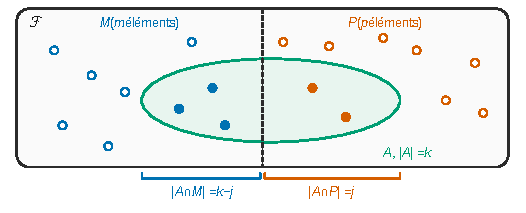
\includegraphics{figures/q09-vandermonde-double-comptage.pdf}
\caption*{Figure 1 --- Double comptage de Vandermonde : une partie A à k éléments
de ℱ = M ⊔ P se coupe en A ∩ M (k − j éléments) et A ∩ P (j éléments)}
\end{figure}

\begin{methode}

Le double comptage : on compte un même ensemble de deux manières, la seconde en le partitionnant selon un paramètre. Une preuve algébrique (coefficient de \(X^k\) dans \((1+X)^m(1+X)^p\)) est aussi correcte, mais l'énoncé oriente vers le dénombrement.

\end{methode}

\hypertarget{question-10}{%
\subsection{Question 10}\label{question-10}}

\begin{indication}{1}

Écrivez le produit \(n(n-1)\cdots(n-k+1)\) comme un quotient de factorielles.

\end{indication}

\hypertarget{solution-9}{%
\subsubsection{Solution}\label{solution-9}}

Si \(k=0\), \(B^n_0=1=\binom n0\).

Si \(1\leqslant k\leqslant n\), le produit \(n(n-1)\cdots(n-k+1)\) compte \(k\) facteurs entiers. Il vaut \(\frac{n!}{(n-k)!}\) :

\equationajustee{\begin{aligned}B^n_k&=\frac{n!}{k!\,(n-k)!}\\&=\binom nk.\end{aligned}}

\textbf{Les deux nombres sont égaux.}

\begin{piege}

Pour \(\lambda\) réel non entier, on ne peut pas écrire \(B^\lambda_\ell\) avec des factorielles : il faut garder la forme « produit descendant sur \(\ell!\) », et ne pas noter \(\binom\lambda\ell\) sans précaution.

\end{piege}

\hypertarget{partie-c-une-famille-de-polynuxf4mes}{%
\section{Partie C --- Une famille de polynômes}\label{partie-c-une-famille-de-polynuxf4mes}}

On travaille avec une base orthonormale \((P_0,\dots,P_n)\) de \(\mathbb R_n[X]\) échelonnée en degré, sans formule explicite. Tout se déduit des deux propriétés (i) et (ii) : degré, orthogonalité à \(\mathbb R_{k-1}[X]\), relation à trois termes, puis localisation des racines par un argument de signe.

\hypertarget{i-premiuxe8res-propriuxe9tuxe9s-des-p_k}{%
\subsection{\texorpdfstring{I -- Premières propriétés des \(P_k\)}{I -- Premières propriétés des P\_k}}\label{i-premiuxe8res-propriuxe9tuxe9s-des-p_k}}

\hypertarget{question-11}{%
\subsection{Question 11}\label{question-11}}

\begin{indication}{1}

La condition (i) enferme \(P_k\) dans \(\mathbb R_k[X]\). Que se passerait-il si \(P_k\) était dans \(\mathbb R_{k-1}[X]\) ?

\end{indication}

\begin{indication}{2}

Argument de dimension.

\end{indication}

\hypertarget{solution-10}{%
\subsubsection{Solution}\label{solution-10}}

Par (i), \(P_k\in\mathrm{Vect}(P_0,\dots,P_k)=\mathbb R_k[X]\), donc \(\deg P_k\leqslant k\).

Pour \(k=0\) : \(P_0\neq0\) (il est de norme \(1\)), donc \(\deg P_0=0\).

Pour \(k\geqslant1\), supposons \(P_k\in\mathbb R_{k-1}[X]\). Par (i) au rang \(k-1\), on a \(\mathbb R_{k-1}[X]=\mathrm{Vect}(P_0,\dots,P_{k-1})\). Ce sous-espace contient alors \(P_0,\dots,P_k\), d'où

\equationajustee{\mathbb R_k[X]=\mathrm{Vect}(P_0,\dots,P_k)\subset\mathbb R_{k-1}[X].}

Cela contredit \(\dim\mathbb R_k[X]=k+1>k=\dim\mathbb R_{k-1}[X]\).

\textbf{Donc \(\deg P_k=k\) pour tout \(k\).}

\begin{piege}

L'énoncé ne décrit pas le procédé de Gram-Schmidt : il en donne deux propriétés, et c'est sur elles seules qu'il faut raisonner.

\end{piege}

\hypertarget{question-12}{%
\subsection{Question 12}\label{question-12}}

\begin{indication}{1}

Réécrivez \(\mathrm{Vect}(1,\dots,X^{k-1})\) à l'aide de (i).

\end{indication}

\hypertarget{solution-11}{%
\subsubsection{Solution}\label{solution-11}}

Par (i), \(\mathrm{Vect}(1,\allowbreak X,\allowbreak \dots,\allowbreak X^{k-1})=\mathrm{Vect}(P_0,\allowbreak \dots,\allowbreak P_{k-1})\). Comme la famille est orthonormale, \(\langle P_k,P_j\rangle=0\) pour tout \(j\leqslant k-1\).

Par linéarité, \(P_k\) est orthogonal à toute combinaison linéaire des \(P_j\), \(j\leqslant k-1\) :

\equationajustee{P_k\in\mathrm{Vect}(1,X,\dots,X^{k-1})^\perp.}

\begin{methode}

Être orthogonal à un sous-espace équivaut à être orthogonal à une famille génératrice de ce sous-espace (par bilinéarité).

\end{methode}

\hypertarget{question-13}{%
\subsection{Question 13}\label{question-13}}

\begin{indication}{1}

Décomposez \(Q\) dans la base orthonormale : ses coordonnées sont des produits scalaires.

\end{indication}

\begin{indication}{2}

Le degré de \(Q\) élimine les coordonnées d'indice \(>k\), l'orthogonalité celles d'indice \(<k\).

\end{indication}

\hypertarget{solution-12}{%
\subsubsection{Solution}\label{solution-12}}

Comme \(\deg Q=k\), on a \(Q\in\mathbb R_k[X]=\mathrm{Vect}(P_0,\dots,P_k)\), et, la famille étant orthonormale,

\equationajustee{Q=\sum_{j=0}^k\langle Q,P_j\rangle P_j.}

Soit \(j\leqslant k-1\). Le polynôme \(P_j\) est de degré \(j\) (Q11), donc appartient à \(\mathbb R_{k-1}[X]\). Comme \(Q\perp\mathbb R_{k-1}[X]\), on a \(\langle Q,P_j\rangle=0\).

Il reste \(Q=\alpha_kP_k\) avec \(\alpha_k=\langle Q,P_k\rangle\), non nul car \(Q\neq0\).

\begin{methode}

C'est une propriété d'unicité : à un scalaire près, il n'existe qu'un polynôme de degré \(k\) orthogonal à \(\mathbb R_{k-1}[X]\). Elle permettra d'identifier les polynômes de Jacobi normalisés aux \(P_k\) (Q28).

\end{methode}

\hypertarget{ii-une-relation-entre-p_k-1-p_k-et-p_k1}{%
\subsection{\texorpdfstring{II -- Une relation entre \(P_{k-1}\), \(P_k\) et \(P_{k+1}\)}{II -- Une relation entre P\_\{k-1\}, P\_k et P\_\{k+1\}}}\label{ii-une-relation-entre-p_k-1-p_k-et-p_k1}}

\hypertarget{question-14}{%
\subsection{Question 14}\label{question-14}}

\begin{indication}{1}

\(P_{k+1}\) et \(XP_k\) ont le même degré : choisissez \(a_k\) pour faire disparaître le terme de plus haut degré.

\end{indication}

\hypertarget{solution-13}{%
\subsubsection{Solution}\label{solution-13}}

Notons \(\lambda_j\) le coefficient dominant de \(P_j\), non nul par Q11.

Les polynômes \(P_{k+1}\) et \(XP_k\) sont de degré \(k+1\). Leurs coefficients dominants sont \(\lambda_{k+1}\) et \(\lambda_k\). En posant

\equationajustee{a_k=\frac{\lambda_{k+1}}{\lambda_k},}

le coefficient de \(X^{k+1}\) dans \(P_{k+1}-a_kXP_k\) vaut \(\lambda_{k+1}-a_k\lambda_k=0\). Donc \(\deg(P_{k+1}-a_kXP_k)\leqslant k\).

\hypertarget{question-15}{%
\subsection{Question 15}\label{question-15}}

\begin{indication}{1}

Décomposez \(R=P_{k+1}-a_kXP_k\) dans la base \((P_0,\dots,P_k)\) et montrez que la plupart des coordonnées sont nulles.

\end{indication}

\begin{indication}{2}

Pour ce produit scalaire, la multiplication par \(X\) « passe d'un côté à l'autre » : comparez \(\langle XA,B\rangle\) et \(\langle A,XB\rangle\).

\end{indication}

\hypertarget{solution-14}{%
\subsubsection{Solution}\label{solution-14}}

\(R=P_{k+1}-a_kXP_k\) est dans \(\mathbb R_k[X]=\mathrm{Vect}(P_0,\dots,P_k)\) par Q14, donc \(R=\sum_{j=0}^k\langle R,P_j\rangle P_j\).

Pour tous \(A,B\in\mathbb R[X]\) :

\equationajustee{\begin{aligned}\langle XA,B\rangle&=\int_{-1}^1w(t)\,tA(t)B(t)\,dt\\&=\langle A,XB\rangle.\end{aligned}}

Soit \(j\in\{0,\dots,k-2\}\) (il n'y a rien à faire si \(k=1\)). Alors

\equationajustee{\begin{aligned}\langle R,P_j\rangle&=\langle P_{k+1},P_j\rangle-a_k\langle XP_k,P_j\rangle\\&=0-a_k\langle P_k,XP_j\rangle\\&=0,\end{aligned}}

car \(j\neq k+1\). De plus, \(XP_j\) est de degré \(j+1\leqslant k-1\), donc orthogonal à \(P_k\) (Q12).

Il ne reste que les indices \(k-1\) et \(k\). Avec \(b_k=\langle R,P_k\rangle\) et \(c_k=\langle R,P_{k-1}\rangle\) :

\equationajustee{P_{k+1}=(a_kX+b_k)P_k+c_kP_{k-1}.}

\begin{methode}

La preuve n'utilise que l'orthogonalité et l'échelonnement des degrés. Elle vaut donc pour toute famille orthogonale (non nécessairement normée) avec \(\deg P_j=j\), les coordonnées devenant \(\langle R,P_j\rangle/\|P_j\|^2\). C'est ce qui permettra de l'appliquer aux \(L_k\) en partie E.

\end{methode}

\hypertarget{iii-racines-des-polynuxf4mes-p_k}{%
\subsection{\texorpdfstring{III -- Racines des polynômes \(P_k\)}{III -- Racines des polynômes P\_k}}\label{iii-racines-des-polynuxf4mes-p_k}}

\hypertarget{question-16}{%
\subsection{Question 16}\label{question-16}}

\begin{indication}{1}

Combien de racines, comptées avec multiplicité, un polynôme non nul de degré \(k\) peut-il avoir ?

\end{indication}

\hypertarget{solution-15}{%
\subsubsection{Solution}\label{solution-15}}

\(P_k\) est non nul de degré \(k\) (Q11) : il admet au plus \(k\) racines réelles comptées avec multiplicité, et celles de \(]-1,1[\) en font partie. \textbf{Donc \(m\leqslant k\).}

\hypertarget{question-17}{%
\subsection{Question 17}\label{question-17}}

\begin{indication}{1}

\(S\) divise \(P_k\). Que dire du quotient sur \(]-1,1[\) ?

\end{indication}

\begin{indication}{2}

Le quotient n'a pas de racine dans \(]-1,1[\) : le théorème des valeurs intermédiaires fixe son signe. Écrivez ensuite \(P_kS\) à l'aide de \(S^2\).

\end{indication}

\hypertarget{solution-16}{%
\subsubsection{Solution}\label{solution-16}}

Si \(\mathcal R=\varnothing\), on a \(S=1\) et \(P_kS=P_k\). C'est une fonction continue qui ne s'annule pas sur l'intervalle \(]-1,1[\) : par le théorème des valeurs intermédiaires, elle y garde un signe strict constant.

Supposons \(m\geqslant1\). Les racines de \(P_k\) dans \(]-1,1[\) sont exactement \(x_1,\dots,x_m\), répétées selon leur multiplicité. Donc \(S\) divise \(P_k\).

Écrivons \(P_k=ST\), où \(T\) n'a aucune racine dans \(]-1,1[\). Chaque racine y a en effet été « consommée » par \(S\) à l'ordre exact de sa multiplicité.

La fonction \(T\) est continue et ne s'annule pas sur l'intervalle \(]-1,1[\). Par le théorème des valeurs intermédiaires, elle y garde un signe strict constant \(\varepsilon\in\{-1,1\}\). Alors

\equationajustee{P_k(x)S(x)=S(x)^2\,T(x),}

\textbf{donc \(P_kS\) est de signe constant sur \(]-1,1[\)}, celui de \(T\). Il ne s'y annule qu'en \(x_1,\dots,x_m\).

\begin{figure}[H]
\centering
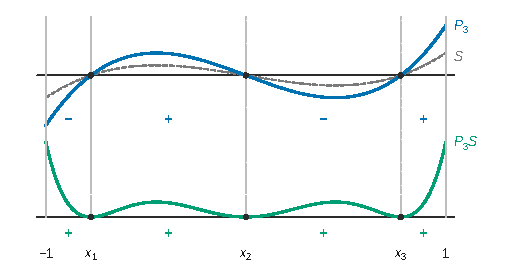
\includegraphics{figures/q17-signe-pk-s.pdf}
\caption*{Figure 2 --- Cas k = 3 : P₃ et S changent de signe aux mêmes racines x₁,
x₂, x₃ ; leur produit P₃S garde un signe constant (allure, échelles
verticales arbitraires)}
\end{figure}

\begin{piege}

Le signe n'est pas forcément positif : c'est celui de \(T\). Et la divisibilité de \(P_k\) par \(S\) exige que les multiplicités soient respectées, d'où la précision de l'énoncé.

\end{piege}

\hypertarget{question-18}{%
\subsection{Question 18}\label{question-18}}

\begin{indication}{1}

Une fonction continue de signe constant, non identiquement nulle, a une intégrale non nulle. Reprenez l'argument de segment de Q4.

\end{indication}

\hypertarget{solution-17}{%
\subsubsection{Solution}\label{solution-17}}

Soit \(\varphi=\varepsilon\,w\,P_kS\), continue et positive sur \(]-1,1[\). L'intégrale suivante converge par Q3 :

\equationajustee{\varepsilon\langle P_k,S\rangle=\int_{-1}^1\varphi.}

Supposons \(\langle P_k,S\rangle=0\). L'argument de Q4, appliqué sur tout segment \([c,d]\subset]-1,1[\), donnerait \(\varphi=0\) sur \(]-1,1[\). Puisque \(w>0\), on aurait \(P_kS=0\) sur cet intervalle.

Le polynôme \(P_kS\) aurait une infinité de racines, donc serait nul. Comme \(S\neq0\), cela imposerait \(P_k=0\) : c'est absurde. \textbf{Donc \(\langle P_k,S\rangle\neq0\).}

\hypertarget{question-19}{%
\subsection{Question 19}\label{question-19}}

\begin{indication}{1}

Comparez Q18 avec Q12 : quel est le degré de \(S\) ?

\end{indication}

\hypertarget{solution-18}{%
\subsubsection{Solution}\label{solution-18}}

\(S\) est de degré \(m\). Si \(m\leqslant k-1\), alors \(S\in\mathbb R_{k-1}[X]\) et Q12 donne \(\langle P_k,S\rangle=0\), contredisant Q18. Donc \(m\geqslant k\), et avec Q16 :

\equationajustee{m=k.}

\textbf{Toutes les racines de \(P_k\) sont réelles et appartiennent à \(]-1,1[\).}

On peut aller plus loin : ces racines sont simples. Soient \(y_1,\dots,y_r\) les racines distinctes de \(P_k\) dans \(]-1,1[\) de multiplicité impaire. On pose \(U=\prod_{i=1}^r(X-y_i)\), avec \(U=1\) si \(r=0\).

Dans \(P_kU\), toutes les racines situées dans \(]-1,1[\) sont de multiplicité paire. Donc \(P_kU\) ne change pas de signe sur cet intervalle.

Le raisonnement de Q18 donne \(\langle P_k,U\rangle\neq0\), puis Q12 donne \(r\geqslant k\). Ainsi \(P_k\) a \(k\) racines distinctes, toutes simples.

\begin{piege}

Avec le \(S\) de l'énoncé, qui compte les multiplicités, on obtient \(m=k\) mais pas la simplicité. Pour la simplicité, il faut changer de polynôme auxiliaire.

\end{piege}

\hypertarget{partie-d-polynuxf4mes-de-jacobi}{%
\section{Partie D --- Polynômes de Jacobi}\label{partie-d-polynuxf4mes-de-jacobi}}

On construit explicitement des polynômes orthogonaux : on dérive \(k\) fois \(g_k=(1-x)^{\alpha+k}(1+x)^{\beta+k}\) et on divise par le poids. La formule de Leibniz et les coefficients \(B^\lambda_\ell\) donnent la forme polynomiale ; des intégrations par parties répétées donnent l'orthogonalité.

\hypertarget{i-duxe9finition}{%
\subsection{I -- Définition}\label{i-duxe9finition}}

\hypertarget{question-20}{%
\subsection{Question 20}\label{question-20}}

\begin{indication}{1}

Dérivez \(g_1\) comme un produit et factorisez par \((1-x)^\alpha(1+x)^\beta\).

\end{indication}

\hypertarget{solution-19}{%
\subsubsection{Solution}\label{solution-19}}

On a \(g_0(x)=(1-x)^\alpha(1+x)^\beta\) et \(g_1(x)=(1-x)^{\alpha+1}(1+x)^{\beta+1}\). Donc

\equationajustee{\begin{aligned}J_0&=\dfrac{g_0}{(1-x)^\alpha(1+x)^\beta}\\&=1.\end{aligned}}

Puis

\equationajustee{\begin{aligned}g_1'(x)&=-(\alpha+1)(1-x)^\alpha(1+x)^{\beta+1}+(\beta+1)(1-x)^{\alpha+1}(1+x)^\beta\\&=(1-x)^\alpha(1+x)^\beta\big[(\beta-\alpha)-(\alpha+\beta+2)x\big].\end{aligned}}

Comme \(J_1=-\dfrac{g_1'}{2(1-x)^\alpha(1+x)^\beta}\) :

\equationajustee{\begin{aligned}J_0&=1\\J_1&=\frac{(\alpha+\beta+2)X+\alpha-\beta}{2}\end{aligned}}

\begin{methode}

Contrôle : pour \(\alpha=\beta=0\), on trouve \(J_1=X\), qui sera \(L_1\) en partie E.

\end{methode}

\hypertarget{question-21}{%
\subsection{Question 21}\label{question-21}}

\begin{indication}{1}

Calculez les premières dérivées, conjecturez, démontrez par récurrence.

\end{indication}

\begin{indication}{2}

Le point clé de l'hérédité est la relation entre \(B^j_{p+1}\) et \(B^j_p\).

\end{indication}

\hypertarget{solution-20}{%
\subsubsection{Solution}\label{solution-20}}

Soit \(j\in\mathbb R\). Montrons par récurrence sur \(p\) que, sur \(]-1,1[\),

\equationajustee{\frac{d^p}{dx^p}(1-x)^j=(-1)^p\,p!\,B^j_p\,(1-x)^{j-p}.}

Pour \(p=0\) : \(B^j_0=1\), c'est vrai. Si c'est vrai au rang \(p\), en dérivant :

\equationajustee{\frac{d^{p+1}}{dx^{p+1}}(1-x)^j=(-1)^p\,p!\,B^j_p\,(j-p)\,(-1)\,(1-x)^{j-p-1}.}

Or on a, y compris pour \(p=0\) (où \(1!\,B^j_1=j\)) :

\equationajustee{\begin{aligned}(p+1)!\,B^j_{p+1}&=j(j-1)\cdots(j-p)\\&=p!\,B^j_p\,(j-p).\end{aligned}}

D'où le rang \(p+1\) ; par récurrence, pour tout \(p\in\mathbb N\) :

\equationajustee{\frac{d^{p}}{dx^{p}}(1-x)^j=(-1)^p\,p!\,B^j_p\,(1-x)^{j-p}.}

Le même calcul sans le signe donne \(\dfrac{d^p}{dx^p}(1+x)^j=p!\,B^j_p\,(1+x)^{j-p}\).

\hypertarget{question-22}{%
\subsection{Question 22}\label{question-22}}

\begin{indication}{1}

\(g_k\) est un produit de deux facteurs : formule de Leibniz, puis Q21 sur chaque facteur.

\end{indication}

\begin{indication}{2}

Simplifiez \(\binom pi\,i!\,(p-i)!\) et mettez en facteur le poids. Faites-le pour un ordre \(p\leqslant k\) quelconque, cela servira en Q25.

\end{indication}

\hypertarget{solution-21}{%
\subsubsection{Solution}\label{solution-21}}

Pour \(p\in\{0,\dots,k\}\), la formule de Leibniz et Q21 donnent

\equationajustee{g_k^{(p)}(x)=\sum_{i=0}^p\binom pi\Big[(-1)^ii!\,B^{\alpha+k}_i(1-x)^{\alpha+k-i}\Big]\Big[(p-i)!\,B^{\beta+k}_{p-i}(1+x)^{\beta+k-p+i}\Big].}

On utilise \(\binom pi\,i!\,(p-i)!=p!\). On met en facteur \((1-x)^{\alpha+k-p}(1+x)^{\beta+k-p}\) : les exposants restants \(p-i\) et \(i\) sont des entiers positifs. On obtient

\equationajustee{g_k^{(p)}(x)=(1-x)^{\alpha+k-p}(1+x)^{\beta+k-p}\,h_p(x),}

où

\equationajustee{h_p(x)=p!\sum_{i=0}^p(-1)^iB^{\alpha+k}_iB^{\beta+k}_{p-i}(1-x)^{p-i}(1+x)^i}

est polynomiale de degré au plus \(p\). Pour \(p=k\) :

\equationajustee{g_k^{(k)}(x)=k!\,(1-x)^\alpha(1+x)^\beta\sum_{i=0}^k(-1)^iB^{\alpha+k}_iB^{\beta+k}_{k-i}(1-x)^{k-i}(1+x)^i.}

\begin{piege}

Le signe \((-1)^i\) ne porte que sur le facteur \((1-x)^{\alpha+k}\). L'oublier fausse Q23 et Q24.

\end{piege}

\hypertarget{question-23}{%
\subsection{Question 23}\label{question-23}}

\begin{indication}{1}

Reportez dans la définition de \(J_k\) : le poids se simplifie.

\end{indication}

\begin{indication}{2}

Absorbez le signe dans \((1-x)^{k-i}\), puis changez d'indice pour obtenir exactement la forme demandée.

\end{indication}

\hypertarget{solution-22}{%
\subsubsection{Solution}\label{solution-22}}

En reportant Q22 dans la définition de \(J_k\), le poids et \(k!\) se simplifient :

\equationajustee{J_k(x)=\frac1{2^k}\sum_{i=0}^k(-1)^{k+i}B^{\alpha+k}_iB^{\beta+k}_{k-i}(1-x)^{k-i}(1+x)^i.}

Comme \(k+i\) et \(k-i\) ont même parité :

\equationajustee{\begin{aligned}(-1)^{k+i}(1-x)^{k-i}&=\big(-(1-x)\big)^{k-i}\\&=(x-1)^{k-i}.\end{aligned}}

Le changement d'indice \(i\mapsto k-i\) donne

\equationajustee{J_k(x)=\frac1{2^k}\sum_{i=0}^kB^{k+\alpha}_{k-i}B^{k+\beta}_i(x-1)^i(x+1)^{k-i}.}

Ce calcul vaut en fait pour tout \(k\geqslant0\) : pour \(k=1\), il redonne le \(J_1\) de Q20.

\hypertarget{question-24}{%
\subsection{Question 24}\label{question-24}}

\begin{indication}{1}

Chaque terme de la somme est un polynôme de degré \(k\) : quel est son coefficient dominant ?

\end{indication}

\begin{indication}{2}

Vandermonde généralisée avec \(s=k+\alpha\), \(t=k+\beta\) ; vérifiez l'hypothèse \(k\leqslant s+t\). Pour conclure au degré exact, il faut montrer que le coefficient obtenu n'est pas nul.

\end{indication}

\hypertarget{solution-23}{%
\subsubsection{Solution}\label{solution-23}}

Pour chaque \(i\), \((x-1)^i(x+1)^{k-i}\) est polynomial, unitaire, de degré \(k\).

Donc \(J_k\) coïncide sur \(]-1,1[\) avec un polynôme de degré au plus \(k\). Son coefficient de \(X^k\) est

\equationajustee{\lambda_k=\frac1{2^k}\sum_{i=0}^kB^{k+\alpha}_{k-i}B^{k+\beta}_i.}

Pour \(k\geqslant2\), on a \(s+t=2k+\alpha+\beta>2k-2\geqslant k\). La formule de Vandermonde généralisée s'applique et

\equationajustee{\begin{aligned}\lambda_k&=\frac{B^{2k+\alpha+\beta}_k}{2^k}\\&=\frac1{2^k\,k!}\prod_{r=0}^{k-1}(2k+\alpha+\beta-r).\end{aligned}}

Chaque facteur vérifie

\equationajustee{2k+\alpha+\beta-r\geqslant k+1+\alpha+\beta>k-1>0.}

Donc \(\lambda_k>0\) : \textbf{\(J_k\) est polynomiale de degré exactement \(k\), de coefficient dominant \(B^{2k+\alpha+\beta}_k/2^k\).}

Pour \(k=0\) et \(k=1\), Q20 donne directement les valeurs suivantes, conformes à la même formule :

\equationajustee{\begin{aligned}\lambda_0&=1,\\\lambda_1&=\frac{\alpha+\beta+2}2>0.\end{aligned}}

\begin{piege}

Majorer le degré par \(k\) ne suffit pas : la question demande le degré \(k\), donc la non-nullité de \(\lambda_k\), qui repose sur \(\alpha,\beta>-1\).

\end{piege}

\hypertarget{ii-orthogonalituxe9-des-polynuxf4mes-de-jacobi}{%
\subsection{II -- Orthogonalité des polynômes de Jacobi}\label{ii-orthogonalituxe9-des-polynuxf4mes-de-jacobi}}

\hypertarget{question-25}{%
\subsection{Question 25}\label{question-25}}

\begin{indication}{1}

Pour la convergence, utilisez la forme factorisée de Q22 : chaque intégrande est « poids de type Q3 × fonction continue sur \([-1,1]\) ».

\end{indication}

\begin{indication}{2}

Intégrez par parties sur un segment \([u,v]\subset]-1,1[\), puis passez à la limite. Les termes de bord tendent vers \(0\) grâce aux exposants \(\alpha+1>0\), \(\beta+1>0\). Regardez à part le cas \(i=0\).

\end{indication}

\hypertarget{solution-24}{%
\subsubsection{Solution}\label{solution-24}}

\emph{Convergence.} Par Q22,

\equationajustee{\begin{aligned}x^ig_k^{(k)}(x)&=(1-x)^\alpha(1+x)^\beta\,x^ih_k(x),\\x^{i-1}g_k^{(k-1)}(x)&=(1-x)^{\alpha+1}(1+x)^{\beta+1}\,x^{i-1}h_{k-1}(x).\end{aligned}}

La fonction \(x^ih_k\) est continue sur \([-1,1]\). Pour \(i\geqslant1\), il en va de même de \(x^{i-1}h_{k-1}\).

Les exposants \(\alpha,\beta,\alpha+1,\beta+1\) sont \(>-1\) : Q3 donne la convergence des deux intégrales.

\emph{Intégration par parties} sur \([u,v]\subset]-1,1[\) (fonctions de classe \(\mathcal C^1\)) :

\equationajustee{\int_u^vx^ig_k^{(k)}(x)\,dx=\Big[x^ig_k^{(k-1)}(x)\Big]_u^v-i\int_u^vx^{i-1}g_k^{(k-1)}(x)\,dx.}

\emph{Termes de bord.} \(h_{k-1}\) est bornée sur \([-1,1]\) et

\equationajustee{|x^ig_k^{(k-1)}(x)|\leqslant\|h_{k-1}\|_\infty(1-x)^{\alpha+1}(1+x)^{\beta+1}\xrightarrow[x\to\pm1]{}0,}

puisque \(\alpha+1>0\) et \(\beta+1>0\). Les intégrales convergeant, on fait \(u\to-1\) et \(v\to1\) :

\equationajustee{\int_{-1}^1x^ig_k^{(k)}(x)\,dx=-i\int_{-1}^1x^{i-1}g_k^{(k-1)}(x)\,dx.}

\emph{Cas \(i=0\).} La seconde intégrale contient \(x^{-1}\) et diverge en général. Pour \(k=1\), par exemple, l'intégrande est équivalent à \(1/x\) en \(0\).

Le même calcul donne alors

\equationajustee{\begin{aligned}\int_{-1}^1g_k^{(k)}&=\big[g_k^{(k-1)}\big]_{-1}^1\\&=0.\end{aligned}}

C'est la seule lecture cohérente de l'identité (le facteur \(-i\) est nul).

\begin{methode}

Intégration par parties sur un intervalle ouvert : on l'écrit sur un segment, on justifie séparément la convergence des intégrales et la limite des termes de bord, puis on passe à la limite.

\end{methode}

\begin{jury}

Signaler un défaut d'énoncé (ici, le cas \(i=0\)) et l'interpréter de façon raisonnable est préférable à une démonstration de convergence fausse.

\end{jury}

\hypertarget{question-26}{%
\subsection{Question 26}\label{question-26}}

\begin{indication}{1}

Exprimez \(\langle J_k,X^i\rangle\) à l'aide de \(\int x^ig_k^{(k)}\) : le poids se simplifie.

\end{indication}

\begin{indication}{2}

Le calcul de Q25 marche à tout ordre de dérivation \(p\leqslant k\). Itérez-le jusqu'à faire disparaître la puissance de \(x\) ; il reste une intégrale de dérivée.

\end{indication}

\hypertarget{solution-25}{%
\subsubsection{Solution}\label{solution-25}}

Par définition de \(J_k\), on a \(w(t)J_k(t)\,t^i=\dfrac{(-1)^k}{2^kk!}\,t^ig_k^{(k)}(t)\). Donc

\equationajustee{\langle J_k,X^i\rangle=\frac{(-1)^k}{2^kk!}\int_{-1}^1t^ig_k^{(k)}(t)\,dt.}

\emph{Généralisation de Q25.} Pour \(p\in\{1,\dots,k\}\), Q22 donne

\equationajustee{g_k^{(p-1)}=(1-x)^{\alpha+k-p+1}(1+x)^{\beta+k-p+1}h_{p-1},}

avec des exposants \(\geqslant\alpha+1>0\) et \(\geqslant\beta+1>0\). Le raisonnement de Q25 s'applique mot pour mot. Pour \(j\geqslant1\) :

\equationajustee{\int_{-1}^1x^jg_k^{(p)}(x)\,dx=-j\int_{-1}^1x^{j-1}g_k^{(p-1)}(x)\,dx.}

\emph{Itération.} On applique cette relation \(i\) fois, aux ordres \(k,k-1,\dots,k-i+1\). Ils sont tous \(\geqslant1\) car \(i\leqslant k-1\) :

\equationajustee{\int_{-1}^1x^ig_k^{(k)}(x)\,dx=(-1)^i\,i!\int_{-1}^1g_k^{(k-i)}(x)\,dx.}

\emph{Conclusion.} Comme \(k-i\geqslant1\), \(g_k^{(k-i-1)}\) est une primitive de \(g_k^{(k-i)}\). Elle tend vers \(0\) aux deux bornes, car ses exposants sont \(\alpha+i+1>0\) et \(\beta+i+1>0\) :

\equationajustee{\begin{aligned}\int_{-1}^1g_k^{(k-i)}(x)\,dx&=\Big[g_k^{(k-i-1)}\Big]_{-1}^1\\&=0.\end{aligned}}

\textbf{Donc \(\langle J_k,X^i\rangle=0\) pour tout \(i\in\{0,\dots,k-1\}\).}

\begin{piege}

La condition \(i\leqslant k-1\) est essentielle : c'est elle qui laisse une dérivée d'ordre \(\geqslant1\) à intégrer. Pour \(i=k\) le résultat est faux (\(\langle J_k,X^k\rangle>0\)).

\end{piege}

\hypertarget{question-27}{%
\subsection{Question 27}\label{question-27}}

\begin{indication}{1}

« Base » : degrés échelonnés et dimension. « Orthogonale » : décomposez \(J_i\) sur les monômes.

\end{indication}

\hypertarget{solution-26}{%
\subsubsection{Solution}\label{solution-26}}

Par Q24, les \(J_k\) sont non nuls et de degrés \(0,1,\dots,n\) deux à deux distincts : la famille \((J_0,\dots,J_n)\) est libre. Elle compte \(n+1=\dim E\) vecteurs, c'est donc une base de \(E\).

Soit \(0\leqslant i<k\leqslant n\). Le polynôme \(J_i\) est de degré \(i\leqslant k-1\), donc s'écrit \(\sum_{r=0}^{k-1}\mu_rX^r\). Par bilinéarité et Q26 :

\equationajustee{\begin{aligned}\langle J_k,J_i\rangle&=\sum_{r=0}^{k-1}\mu_r\langle J_k,X^r\rangle\\&=0.\end{aligned}}

\textbf{\((J_0,\dots,J_n)\) est une base orthogonale de \(E\).}

\hypertarget{question-28}{%
\subsection{Question 28}\label{question-28}}

\begin{indication}{1}

Comment rend-on unitaire un vecteur non nul ?

\end{indication}

\hypertarget{solution-27}{%
\subsubsection{Solution}\label{solution-27}}

Chaque \(J_k\) est non nul, donc \(\|J_k\|>0\) (produit scalaire défini). La famille

\equationajustee{\Big(\frac{J_0}{\|J_0\|},\dots,\frac{J_n}{\|J_n\|}\Big)}

reste orthogonale et ses vecteurs sont unitaires : \textbf{c'est une base orthonormale de \(E\)}, obtenue en normalisant la base orthogonale de Q27.

Cette base est exactement celle de la partie C. En effet, \(J_k/\|J_k\|\) est de degré \(k\) et orthogonal à \(\mathbb R_{k-1}[X]\). Il vaut donc \(\pm P_k\) par Q13 (les deux sont unitaires).

Écrivons \(X^k=J_k/\lambda_k+(\text{\text{degré}}<k)\). Q26 donne alors

\equationajustee{\langle J_k,X^k\rangle=\frac{\|J_k\|^2}{\lambda_k}>0,}

et la condition (ii) impose le signe \(+\).

\hypertarget{partie-e-le-cas-particulier-alphabeta00}{%
\section{\texorpdfstring{Partie E --- Le cas particulier \((\alpha,\beta)=(0,0)\)}{Partie E --- Le cas particulier (\textbackslash alpha,\textbackslash beta)=(0,0)}}\label{partie-e-le-cas-particulier-alphabeta00}}

Pour \(\alpha=\beta=0\), \(g_k(x)=(1-x^2)^k=(-1)^k(x^2-1)^k\), donc

\equationajustee{\begin{aligned}J_k&=\frac{(-1)^k}{2^kk!}g_k^{(k)}\\&=\frac1{2^kk!}\big[(X^2-1)^k\big]^{(k)}\\&=L_k.\end{aligned}}

Les \(L_k\) sont donc les polynômes de Jacobi eux-mêmes : \textbf{orthogonaux mais pas normés} (\(\|L_0\|^2=\|1\|^2=2\) par Q8), contrairement à ce qu'affirme le préambule. Les raisonnements de Q14--Q15 restent valables pour eux (ils n'utilisent que l'orthogonalité et les degrés).

\hypertarget{i-premiuxe8res-propriuxe9tuxe9s-des-polynuxf4mes-l_k}{%
\subsection{\texorpdfstring{I -- Premières propriétés des polynômes \(L_k\)}{I -- Premières propriétés des polynômes L\_k}}\label{i-premiuxe8res-propriuxe9tuxe9s-des-polynuxf4mes-l_k}}

\hypertarget{question-29}{%
\subsection{Question 29}\label{question-29}}

\begin{indication}{1}

Développez \((X^2-1)^k\) et dérivez \(k\) fois. Contrôlez avec \(L_k(1)\).

\end{indication}

\hypertarget{solution-28}{%
\subsubsection{Solution}\label{solution-28}}

On a \(L_0=1\) et \(L_1=\frac12(X^2-1)'=X\).

Puis \((X^2-1)^2=X^4-2X^2+1\), de dérivée seconde \(12X^2-4\).

De même, \((X^2-1)^3=X^6-3X^4+3X^2-1\), de dérivée troisième \(120X^3-72X\).

Avec \(2^2\cdot2!=8\) et \(2^3\cdot3!=48\) :

\equationajustee{\begin{aligned}L_0&=1\\L_1&=X\\L_2&=\frac{3X^2-1}2\\L_3&=\frac{5X^3-3X}2\end{aligned}}

\begin{methode}

Contrôles gratuits : \(L_k(1)=1\) dans les quatre cas (ce sera Q33), et \(L_k\) a la parité de \(k\) (Q32).

\end{methode}

\hypertarget{question-30}{%
\subsection{Question 30}\label{question-30}}

\begin{indication}{1}

Résolvez, puis vérifiez les trois points de Q19 : racines réelles, dans \(]-1,1[\), au nombre de \(k\).

\end{indication}

\hypertarget{solution-29}{%
\subsubsection{Solution}\label{solution-29}}

\(L_1=X\) : racine \(0\).

\(L_2=\frac{3X^2-1}2\) : racines \(\pm\frac1{\sqrt3}\approx\pm0{,}577\).

\(L_3=\frac{X(5X^2-3)}2\) : racines \(0\) et \(\pm\sqrt{\frac35}\approx\pm0{,}775\).

Dans chaque cas, \(L_k\) a \(k\) racines réelles, simples, toutes dans \(]-1,1[\) : \textbf{\(m=k\), ce qui confirme Q19.}

\begin{figure}[H]
\centering
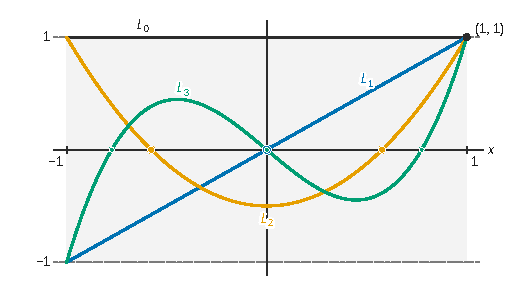
\includegraphics{figures/q30-polynomes-legendre.pdf}
\caption*{Figure 3 --- Polynômes de Legendre L₀ à L₃ entre −1 et 1 : L\_k a k
racines simples, vaut 1 en x = 1 et reste dans la bande
\textbar y\textbar{} ⩽ 1}
\end{figure}

\hypertarget{question-31}{%
\subsection{Question 31}\label{question-31}}

\begin{indication}{1}

Seul le monôme de plus haut degré de \((X^2-1)^k\) contribue au coefficient dominant après \(k\) dérivations.

\end{indication}

\hypertarget{solution-30}{%
\subsubsection{Solution}\label{solution-30}}

On a \((X^2-1)^k=X^{2k}+(\text{termes de \text{degré}}<2k)\). La dérivée \(k\)-ième de \(X^{2k}\) est

\equationajustee{2k(2k-1)\cdots(k+1)X^k=\frac{(2k)!}{k!}X^k.}

Celle d'un monôme de degré \(r<2k\) est de degré \(r-k<k\) (ou nulle). Donc \(\big[(X^2-1)^k\big]^{(k)}\) est de degré \(k\), de coefficient dominant \(\frac{(2k)!}{k!}\neq0\). Ainsi \(\deg L_k=k\), et

\equationajustee{\begin{aligned}\text{coefficient dominant}&=\frac{(2k)!}{2^k(k!)^2}\\&=\frac1{2^k}\binom{2k}k.\end{aligned}}

On retrouve \(B^{2k}_k/2^k\) de Q24, par Q10.

\hypertarget{question-32}{%
\subsection{Question 32}\label{question-32}}

\begin{indication}{1}

\((X^2-1)^k\) est pair. Que fait la dérivation à la parité ?

\end{indication}

\hypertarget{solution-31}{%
\subsubsection{Solution}\label{solution-31}}

Soit \(Q\) pair. On montre par récurrence que \(Q^{(p)}(-x)=(-1)^pQ^{(p)}(x)\). En dérivant cette relation, on obtient en effet

\equationajustee{-Q^{(p+1)}(-x)=(-1)^pQ^{(p+1)}(x).}

Avec \(Q=(X^2-1)^k\) et \(p=k\), puis division par \(2^kk!\) :

\equationajustee{L_k(-X)=(-1)^kL_k(X).}

\textbf{\(L_k\) est pair si \(k\) est pair, impair si \(k\) est impair.}

\hypertarget{question-33}{%
\subsection{Question 33}\label{question-33}}

\begin{indication}{1}

Factorisez \(X^2-1\) et appliquez Leibniz ; en \(x=1\), presque tous les termes s'annulent.

\end{indication}

\begin{indication}{2}

Pour \(L_k(-1)\), inutile de recommencer : utilisez Q32.

\end{indication}

\hypertarget{solution-32}{%
\subsubsection{Solution}\label{solution-32}}

Par Leibniz,

\equationajustee{\big[(X-1)^k(X+1)^k\big]^{(k)}=\sum_{i=0}^k\binom ki\big[(X-1)^k\big]^{(i)}\big[(X+1)^k\big]^{(k-i)}.}

Pour \(i\leqslant k-1\), le facteur \(\big[(X-1)^k\big]^{(i)}=\frac{k!}{(k-i)!}(X-1)^{k-i}\) s'annule en \(1\). Pour \(i=k\), il vaut \(k!\).

En \(x=1\), il reste \(k!\cdot2^k\), d'où \(L_k(1)=1\). Par Q32, \(L_k(-1)=(-1)^kL_k(1)\) :

\equationajustee{\begin{aligned}L_k(1)&=1\\L_k(-1)&=(-1)^k\end{aligned}}

\hypertarget{ii-une-uxe9quation-diffuxe9rentielle-vuxe9rifiuxe9e-par-les-l_k}{%
\subsection{\texorpdfstring{II -- Une équation différentielle vérifiée par les \(L_k\)}{II -- Une équation différentielle vérifiée par les L\_k}}\label{ii-une-uxe9quation-diffuxe9rentielle-vuxe9rifiuxe9e-par-les-l_k}}

\hypertarget{question-34}{%
\subsection{Question 34}\label{question-34}}

\begin{indication}{1}

Dérivez et reconnaissez \(g_k\). Pensez au cas \(k=0\).

\end{indication}

\hypertarget{solution-33}{%
\subsubsection{Solution}\label{solution-33}}

Pour \(k\geqslant1\), \(g_k'(x)=-2kx(1-x^2)^{k-1}\), donc \((1-x^2)g_k'(x)=-2kx(1-x^2)^k\).

Pour \(k=0\), \(g_0'=0\). Dans tous les cas :

\equationajustee{(1-x^2)g_k'(x)=-2kx\,g_k(x).}

\hypertarget{question-35}{%
\subsection{Question 35}\label{question-35}}

\begin{indication}{1}

Dérivez la relation de Q34 un certain nombre de fois par Leibniz. Combien de fois faut-il dériver pour faire apparaître \(g_k^{(k)}\), \(g_k^{(k+1)}\) et \(g_k^{(k+2)}\) ?

\end{indication}

\begin{indication}{2}

Dans chaque Leibniz, un facteur est un polynôme de petit degré : seuls deux ou trois termes subsistent. Reliez enfin \(g_k^{(k)}\) à \(L_k\).

\end{indication}

\hypertarget{solution-34}{%
\subsubsection{Solution}\label{solution-34}}

Notons \(u=g_k\), de sorte que \((1-x^2)u'+2kxu=0\) sur \(]-1,1[\). Dérivons \(k+1\) fois.

On a \((1-x^2)'=-2x\) et \((1-x^2)''=-2\), et les dérivées suivantes sont nulles :

\equationajustee{\big[(1-x^2)u'\big]^{(k+1)}=(1-x^2)u^{(k+2)}-2(k+1)x\,u^{(k+1)}-2\binom{k+1}2u^{(k)},}

avec \(2\binom{k+1}2=k(k+1)\). De même :

\equationajustee{\big[2kxu\big]^{(k+1)}=2k\big(xu^{(k+1)}+(k+1)u^{(k)}\big).}

En sommant :

\equationajustee{(1-x^2)u^{(k+2)}-2x\,u^{(k+1)}+k(k+1)u^{(k)}=0.}

Or \(u^{(k)}=g_k^{(k)}=(-1)^k2^kk!\,L_k\). En divisant par cette constante non nulle :

\equationajustee{(1-x^2)L_k''-2xL_k'+k(k+1)L_k=0\quad\text{sur }]-1,1[.}

\begin{methode}

Multiplier par \(1-x^2\) en Q34 donne une relation à coefficients polynomiaux, que Leibniz dérive à un ordre quelconque en ne gardant que quelques termes. C'est la technique standard pour obtenir l'équation différentielle d'une famille définie par une formule de Rodrigues.

\end{methode}

\hypertarget{iii-une-majoration-des-l_k-sur--11}{%
\subsection{\texorpdfstring{III -- Une majoration des \(L_k\) sur \([-1,1]\)}{III -- Une majoration des L\_k sur {[}-1,1{]}}}\label{iii-une-majoration-des-l_k-sur--11}}

\hypertarget{question-36}{%
\subsection{Question 36}\label{question-36}}

\begin{indication}{1}

Dérivez \(f_k\) ; un terme en \(L_k''\) apparaît, dont on ne connaît pas le signe.

\end{indication}

\begin{indication}{2}

Éliminez \((1-x^2)L_k''\) grâce à l'équation de Q35. Remarquez aussi que \(f_k\) n'est pas définie pour toutes les valeurs de \(k\).

\end{indication}

\hypertarget{solution-35}{%
\subsubsection{Solution}\label{solution-35}}

\(f_k\) n'est définie que pour \(k\geqslant1\) (dénominateur \(k(k+1)\)). Pour \(x\in[0,1]\) :

\equationajustee{\begin{aligned}f_k'(x)&=2L_kL_k'+\frac{1}{k(k+1)}\Big(-2xL_k'^2+2(1-x^2)L_k'L_k''\Big)\\&=2L_kL_k'+\frac{2L_k'}{k(k+1)}\Big[(1-x^2)L_k''-xL_k'\Big].\end{aligned}}

L'équation de Q35 est une égalité entre fonctions polynomiales sur \(]-1,1[\), donc sur \(\mathbb R\). Elle donne \((1-x^2)L_k''=2xL_k'-k(k+1)L_k\), d'où

\equationajustee{(1-x^2)L_k''-xL_k'=xL_k'-k(k+1)L_k.}

En reportant, les termes en \(L_kL_k'\) se compensent :

\equationajustee{f_k'(x)=\frac{2x}{k(k+1)}\,L_k'(x)^2\geqslant0\quad\text{sur }[0,1].}

\textbf{\(f_k\) est croissante sur \([0,1]\).}

\begin{piege}

L'équation de Q35 est établie sur \(]-1,1[\) ; pour l'utiliser en \(x=1\), on invoque le prolongement des identités polynomiales (ou la continuité).

\end{piege}

\hypertarget{question-37}{%
\subsection{Question 37}\label{question-37}}

\begin{indication}{1}

Comparez \(L_k^2\) et \(f_k\) sur \([0,1]\), puis utilisez la croissance et la valeur en \(1\).

\end{indication}

\begin{indication}{2}

Pour \([-1,0]\), une symétrie suffit.

\end{indication}

\hypertarget{solution-36}{%
\subsubsection{Solution}\label{solution-36}}

Pour \(k=0\), \(L_0=1\) et le résultat est immédiat. Soit \(k\geqslant1\) et \(x\in[0,1]\). Comme \(1-x^2\geqslant0\),

\equationajustee{\begin{aligned}L_k(x)^2&\leqslant f_k(x)\\&\leqslant f_k(1)\\&=L_k(1)^2+0\\&=1,\end{aligned}}

par Q36 puis Q33 : le facteur \(1-x^2\) annule le terme en \(L_k'\) en \(x=1\). Donc \(|L_k(x)|\leqslant1\) sur \([0,1]\).

Pour \(x\in[-1,0]\), \(|L_k(x)|=|L_k(-x)|\leqslant1\) par Q32.

\textbf{Ainsi \(|L_k(x)|\leqslant1\) pour tout \(x\in[-1,1]\).}

\begin{methode}

Fonction auxiliaire « énergie » : \(f_k\) combine \(L_k^2\) et \(L_k'^2\) de sorte que l'équation différentielle rende sa dérivée de signe connu. On majore alors \(L_k^2\) par la valeur de \(f_k\) en un point où elle est connue.

\end{methode}

\hypertarget{iv-relation-entre-l_k-1-l_k-et-l_k1}{%
\subsection{\texorpdfstring{IV -- Relation entre \(L_{k-1}\), \(L_k\) et \(L_{k+1}\)}{IV -- Relation entre L\_\{k-1\}, L\_k et L\_\{k+1\}}}\label{iv-relation-entre-l_k-1-l_k-et-l_k1}}

\hypertarget{question-38}{%
\subsection{Question 38}\label{question-38}}

\begin{indication}{1}

Dans Q14, \(a_k\) est un quotient de coefficients dominants ; ceux des \(L_k\) sont connus par Q31.

\end{indication}

\hypertarget{solution-37}{%
\subsubsection{Solution}\label{solution-37}}

La relation de Q14 vaut pour la famille orthogonale échelonnée \((L_j)\) (voir le préambule de la partie E). Le réel \(a_k\) y est le quotient des coefficients dominants de \(L_{k+1}\) et \(L_k\) :

\equationajustee{\begin{aligned}a_k&=\frac{(2k+2)!}{2^{k+1}((k+1)!)^2}\cdot\frac{2^k(k!)^2}{(2k)!}\\&=\frac{(2k+2)(2k+1)}{2}\cdot\frac1{(k+1)^2}\\&=\frac{2k+1}{k+1}.\end{aligned}}

\begin{piege}

Si l'on prenait l'énoncé au pied de la lettre (polynômes orthonormés \(P_k=\sqrt{\frac{2k+1}2}L_k\)), on obtiendrait un autre \(a_k\). Seule la lecture « \(a_k\) relatif aux \(L_k\) » est cohérente avec Q39.

\end{piege}

\hypertarget{question-39}{%
\subsection{Question 39}\label{question-39}}

\begin{indication}{1}

Partez de la relation à trois termes de Q15 avec le \(a_k\) de Q38. Il reste deux constantes.

\end{indication}

\begin{indication}{2}

Une parité élimine \(b_k\) ; une valeur particulière connue des \(L_j\) donne \(c_k\).

\end{indication}

\hypertarget{solution-38}{%
\subsubsection{Solution}\label{solution-38}}

Par Q15 (valable pour la famille orthogonale \((L_j)\)), il existe \((b_k,c_k)\) tels que

\equationajustee{L_{k+1}=(a_kX+b_k)L_k+c_kL_{k-1},}

avec, par Q38,

\equationajustee{a_k=\frac{2k+1}{k+1}.}

\emph{Calcul de \(b_k\).} Par Q32, les polynômes \(L_{k+1}\), \(XL_k\) et \(L_{k-1}\) ont la parité de \(k+1\).

Donc \(b_kL_k=L_{k+1}-a_kXL_k-c_kL_{k-1}\) a la parité de \(k+1\), tout en ayant celle de \(k\).

Un polynôme à la fois pair et impair est nul. Comme \(L_k\neq0\), on obtient \(b_k=0\).

\emph{Calcul de \(c_k\).} En \(x=1\), Q33 donne \(1=a_k+c_k\), donc

\equationajustee{\begin{aligned}c_k&=1-\frac{2k+1}{k+1}\\&=-\frac k{k+1}.\end{aligned}}

\equationajustee{L_{k+1}=\frac{2k+1}{k+1}XL_k-\frac k{k+1}L_{k-1}.}

Vérification pour \(k=1\) : \(\frac32X^2-\frac12=L_2\).

\begin{methode}

Pour identifier des constantes dans une relation polynomiale, parité et valeurs particulières sont souvent plus rapides qu'un calcul de produits scalaires.

\end{methode}

\hypertarget{v-un-duxe9veloppement-en-suxe9rie-entiuxe8re-faisant-intervenir-les-l_k}{%
\subsection{\texorpdfstring{V -- Un développement en série entière faisant intervenir les \(L_k\)}{V -- Un développement en série entière faisant intervenir les L\_k}}\label{v-un-duxe9veloppement-en-suxe9rie-entiuxe8re-faisant-intervenir-les-l_k}}

\hypertarget{question-40}{%
\subsection{Question 40}\label{question-40}}

\begin{indication}{1}

Utilisez la majoration de Q37 et la définition du rayon de convergence.

\end{indication}

\hypertarget{solution-39}{%
\subsubsection{Solution}\label{solution-39}}

Fixons \(x\in[-1,1]\). Par Q37, étendue à tout \(k\in\mathbb N\) comme l'énoncé l'autorise, on a \(|L_k(x)|\leqslant1\).

Soit \(r\in[0,1[\). Alors \(|L_k(x)r^k|\leqslant1\) : la suite \((L_k(x)r^k)\) est bornée. Le rayon \(R_x\) vérifie donc \(R_x\geqslant r\). Ceci valant pour tout \(r<1\) :

\equationajustee{R_x\geqslant1.}

En particulier \(S(t)\) est bien définie pour \(t\in]-1,1[\).

\begin{piege}

On demande une minoration du rayon, pas sa valeur. Ne pas affirmer \(R_x=1\) sans preuve.

\end{piege}

\hypertarget{question-41}{%
\subsection{Question 41}\label{question-41}}

\begin{indication}{1}

Dérivez \(S\) terme à terme et écrivez \(S'(t)=\sum(k+1)L_{k+1}(x)t^k\).

\end{indication}

\begin{indication}{2}

Injectez la relation de Q39 écrite sous la forme \((k+1)L_{k+1}=\dots\) ; vérifiez qu'elle vaut aussi pour \(k=0\). Exprimez chaque somme obtenue avec \(S\) et \(S'\) par décalage d'indice.

\end{indication}

\hypertarget{solution-40}{%
\subsubsection{Solution}\label{solution-40}}

Le rayon étant \(\geqslant1\), \(S\) est dérivable sur \(]-1,1[\) et

\equationajustee{\begin{aligned}S'(t)&=\sum_{k\geqslant1}kL_k(x)t^{k-1}\\&=\sum_{k\geqslant0}(k+1)L_{k+1}(x)t^k.\end{aligned}}

On utilise la relation suivante :

\equationajustee{(k+1)L_{k+1}=(2k+1)xL_k-kL_{k-1}.}

Elle vaut pour \(k\geqslant1\) par Q39. Pour \(k=0\), elle se réduit à \(L_1=xL_0\), le terme \(kL_{k-1}\) étant nul. Toutes les séries ci-dessous ont un rayon \(\geqslant1\) (multiplier les coefficients par \(k\) ne change pas le rayon), on peut donc séparer :

\equationajustee{S'(t)=2x\sum_{k\geqslant0}kL_kt^k+x\sum_{k\geqslant0}L_kt^k-\sum_{k\geqslant1}kL_{k-1}t^k.}

Or \(\sum_{k\geqslant0}kL_kt^k=tS'(t)\) et, avec \(j=k-1\),

\equationajustee{\begin{aligned}\sum_{k\geqslant1}kL_{k-1}t^k&=\sum_{j\geqslant0}(j+1)L_jt^{j+1}\\&=t\big(tS'(t)+S(t)\big).\end{aligned}}

D'où

\equationajustee{S'=2xtS'+xS-t^2S'-tS,}

c'est-à-dire

\equationajustee{(1-2tx+t^2)S'(t)+(t-x)S(t)=0.}

\begin{methode}

Contrôle sur le terme constant : en \(t=0\), on trouve \(S'(0)=xS(0)\), c'est-à-dire \(L_1(x)=x\).

\end{methode}

\hypertarget{question-42}{%
\subsection{Question 42}\label{question-42}}

\begin{indication}{1}

C'est une équation différentielle linéaire d'ordre 1. Vérifiez d'abord que \(1-2tx+t^2\) ne s'annule pas sur \(]-1,1[\).

\end{indication}

\begin{indication}{2}

Plutôt que de diviser par \(S\), étudiez le produit de \(S\) par une fonction bien choisie, dont la dérivée est nulle. La constante se trouve en \(t=0\).

\end{indication}

\hypertarget{solution-41}{%
\subsubsection{Solution}\label{solution-41}}

Posons \(\varphi(t)=1-2tx+t^2\). On a

\equationajustee{\varphi(t)=(t-x)^2+(1-x^2).}

Si \(|x|<1\), \(\varphi(t)\geqslant1-x^2>0\). Si \(x=\pm1\), \(\varphi(t)=(t\mp1)^2>0\) pour \(t\in]-1,1[\).

Donc \(\varphi>0\) sur \(]-1,1[\), et \(\varphi'(t)=2(t-x)\).

Soit \(H=S\sqrt\varphi\), dérivable sur \(]-1,1[\) :

\equationajustee{\begin{aligned}H'(t)&=S'(t)\sqrt{\varphi(t)}+S(t)\frac{\varphi'(t)}{2\sqrt{\varphi(t)}}\\&=\frac{\varphi(t)S'(t)+(t-x)S(t)}{\sqrt{\varphi(t)}}\\&=0\end{aligned}}

par Q41. \(H\) est donc constante sur l'intervalle \(]-1,1[\). Sa valeur est \(H(0)=S(0)\sqrt{\varphi(0)}=L_0(x)=1\). Ainsi, pour tout \(t\in]-1,1[\) :

\equationajustee{\sum_{k=0}^{+\infty}L_k(x)t^k=\frac1{\sqrt{1-2tx+t^2}}.}

\begin{methode}

Pour \(y'=a(t)y\), multiplier par \(e^{-A(t)}\) (ici \(\sqrt\varphi\)) et montrer que le produit est constant évite toute division par la fonction inconnue.

\end{methode}

\begin{piege}

Les cas \(x=\pm1\) sont ceux où le trinôme peut s'annuler ; il s'annule en \(t=\pm1\), hors de l'intervalle ouvert. Il faut le dire. Contrôle : pour \(x=1\), on retrouve \(\sum t^k=\frac1{1-t}\), cohérent avec \(L_k(1)=1\).

\end{piege}

\hypertarget{bilan}{%
\section{Bilan}\label{bilan}}

\textbf{Méthodes à retenir.}

\begin{itemize}
\tightlist
\item
  Intégrabilité d'un poids singulier aux bornes : couper l'intervalle, borner le facteur continu sur un segment, comparer à une intégrale de Riemann (Q3).
\item
  Caractère défini d'un produit scalaire intégral sur un intervalle ouvert : se ramener à des segments intérieurs (Q4, Q18).
\item
  Polynômes orthogonaux échelonnés : orthogonalité à \(\mathbb R_{k-1}[X]\), unicité à un scalaire près, relation à trois termes grâce à \(\langle XA,B\rangle=\langle A,XB\rangle\) (Q12--Q15).
\item
  Racines dans l'intervalle d'orthogonalité : argument de signe avec le polynôme auxiliaire \(S\) (Q17--Q19).
\item
  Formule de Leibniz quand un facteur est polynomial de petit degré : la somme se réduit à deux ou trois termes (Q33, Q35).
\item
  Intégrations par parties répétées sur un intervalle ouvert, avec annulation des termes de bord (Q25--Q26).
\item
  Utiliser une équation différentielle pour éliminer une dérivée seconde (Q36) ou pour identifier la somme d'une série entière (Q41--Q42).
\end{itemize}

\textbf{Prérequis à revoir.} Critère de Riemann ; théorème de changement de variable pour les intégrales impropres ; multiplicité des racines et divisibilité ; dérivation terme à terme des séries entières ; résolution d'une équation différentielle linéaire d'ordre 1.

\textbf{Questions classiques transposables.} La démonstration que les racines d'un polynôme orthogonal sont réelles, simples et dans l'intervalle (Q16--Q19) vaut pour tout poids positif ; la récurrence à trois termes (Q14--Q15) et la formule de Rodrigues avec orthogonalité par intégrations par parties (Q25--Q26) se retrouvent pour les polynômes de Tchebychev, de Laguerre ou d'Hermite ; la fonction génératrice des polynômes de Legendre (Q42) est un exemple type d'identification d'une série entière par une équation différentielle.

\end{document}
